\documentclass[letterpaper,10pt]{article}
\usepackage{graphicx}
\usepackage{amsmath,amssymb,array,calc,epsfig,rotating,bm, hyperref}
\usepackage[sort]{cite}
\usepackage{psfrag,verbatim}
\usepackage{mathtools}
\usepackage[margin=1in]{geometry}

\def\code#1{\texttt{#1}}

%opening
\title{Unsupervised learning on causal sets with variational autencoders}
\author{Anton van Niekerk}

\begin{document}

\maketitle

\begin{abstract}
I apply a variational autencoder to the causal matrix for causal sets embedded in $2$, $3$, and $4$ dimensional causal diamonds, 
and find that the latent variables successfully separate the causal sets by dimension.
\end{abstract}


\section{Introduction}

\subsection{Causal Sets}

When one typically thinks of the spacetime (time being thought of as a distinct ``direction'' to the three spatial dimensions we live in), 
the tendency in physics is to represent it as a a continuous space, i.e., as a four dimensional real
space where one of the dimensions is associated to the time direction.  In that case, for every point in the spacetime, there are infinitely many other 
points arbitrarily close to that point (in other words the spacetime is continuous).

When one tries to combine gravity, which in Einstein's theory of general relativity is the geometric curvature of spacetime, 
with quantum mechanics, the theory which describes elementary particles such as electrons and quarks, any quantity one cares about, such as the 
energy at which particles interact with gravity, gives the answer of infinity.  While physicists have found ways to deal with infinite answers in other 
theories, such as quantum electrodynamics and find out the correct finite answer to their questions, none of these methods work for quantum gravity, and 
the infinities remain.  Clearly, some new assumptions about nature are needed to successfully combine gravity and quantum mechanics.

One attempt to do this was through {\it causal sets} \cite{causalsets}.  A causal set is a discrete version of spacetime, meaning that there are finite gaps 
between any spacetime point and the nearest other point to it.  Because the distances between points in a causal set is finite, rather than infinitesimal 
as in the usual description of spacetime, quantum gravity in causal sets are free of the infinite answers mentioned above.

\begin{figure}
\begin{center}
  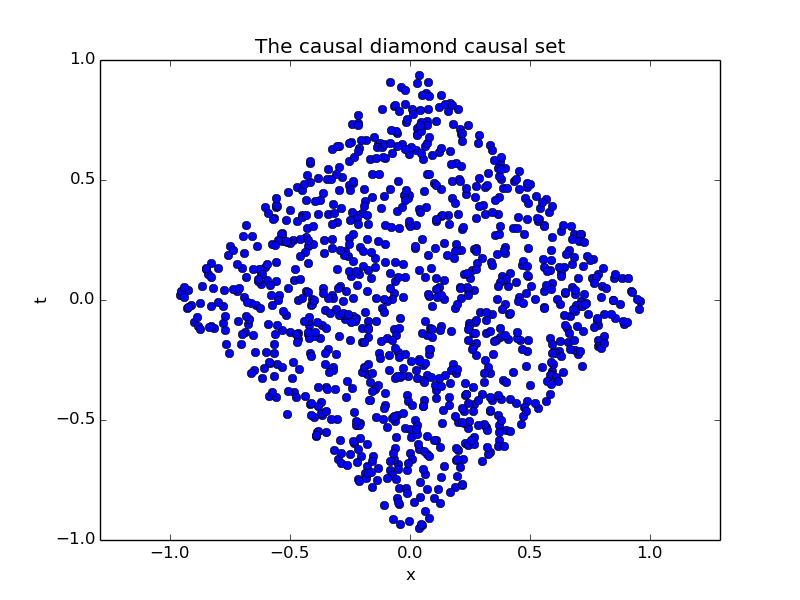
\includegraphics[width=5in]{causaldiamond2d.png}
\end{center}
  \caption{
A $2$-dimensional causal diamond causal set with $1000$ spacetime points.  
The axes are scaled such that something moving at the speed of light would travel at a 
$45$ degree angle with the vertical.  Since the sides of the causal diamond are light rays, its sides are also at $45$ degree angles.} \label{causet2d}
\end{figure}

One way to create a causal set that approximates a continuous spacetime, is to ``sprinkle'' points at random into the continuum spacetime, see figure 
\ref{causet2d} for a two-dimensional example.  Because the points are randomly sprinkled, there is on average the same number of points per small volume 
of the spacetime.  Also, this random sprinkling ensures that the causal set satisfies the same symmetries as the continuum spacetime.  As an example, if a 
sphere is sprinkled with random points, since the sphere looks the same under any rotation, so will the random sprinkling under the same rotation.

A final property of causal sets that will be important is that the points in the set only ``know'' about points that can communicate with them.  From 
special relativity we know that no information can travel faster than the speed of light, so only points that can send a signal at or slower than the 
speed of light to some future point will be ``connected'' to the future point.  In physics this property is called {\it causality}, hence the name 
``causal sets''.

The causal connections of the points in the causal set are encoded in the {\it causal matrix} $c_{mn}$, where
\begin{equation}
 c_{mn} = \begin{cases}
      1 & \text{if point $m$ is to the past of point $n$, and can send a message to point $n$}\\
      0 & \text{otherwise.}
    \end{cases} 
\end{equation}
It turns out that all the properties of the continuum spacetime\footnote{except for volume and distance, since scale is an independent 
parameter.} (such as its symmetries and shape) can be derived from the causal matrix.  One can therefore view a causal set as a discrete representation 
of a continuum spacetime, which can a useful tool to do certain kinds of calculations more easily.

Certain calculations on causal sets can be extremely costly, requiring operations such as finding the eigenvalues of matrices of the same order as the 
causal matrix.  This has to some extent hampered research in this field by requiring the sizes of causal sets to be not more than a few thousand points.  
The motivation of this project is for it to be a first step in using machine learning in aiding causal set research.  If a neural network can be trained
to recognize details or estimate quantities in causal sets, it could potentially help accelerate certain computational research programs in the field.

If the causal connections between the causal set points are drawn as lines, the causal set can be viewed as a graph.  This graphlike nature means that 
one might want to look for things like clusters of vertices in the graph, or perhaps more relevantly, the number of connections per vertex.

\subsection{Variational Autoencoders} \label{vaesection}

A variational autoencoder \cite{vae} (VAE) is a type of neural network, which is trained to approximately map the input back to itself.  As such, 
VAE's are an example of unsupervised learning, since it doesn't require labels to train the network parameters.

When represented by the size of the hidden layers of the neural network, a VAE typically has an hour-glass shape.  That is, starting with the input layer, 
each subsequent hidden layer has smaller dimensions than the previous layer, until one reaches a layer with the smallest dimension.  
The elements of this hidden layer are known as the {\it latent variables}, and represent an {\it encoding} of the input that is of reduced dimension.  
The hidden layers following the layer of latent variables each have greater dimension than the previous layers, until one reaches the output layer which 
has the same dimension as the input layer.

The layers of the VAE up to and including the latent layer are known collectively as the {\it encoder}, and the layers after the latent variables 
up to the output are known as the {\it decoder}.  This separation is useful, as the encoder can be used for a low-dimensional representation of 
the input data and used as an unsupervised clustering algorithm, while the decoder can be used to generate artificial data that nonetheless looks 
realistic (see e.g. \cite{vaemnist} for examples of encoders and decoders using the MNIST \cite{mnist} dataset).  I will be primarily interested in 
the encoder part of the VAE for now.

One final property of a variational autoencoder is that it implements {\it variational Bayes}, which means that when training the neural network, 
the input data is assumed to be from a random distribution.  This is represented by the fact that on training the network, a random error is added to 
the latent variable \cite{vae, kerasauto}.  The latent variables are represented by the vector $z_{\text mean}$, and the variance of 
random error is represented by the vector $z_{\text log var}$.  Both of these vectors are (independently) densely connected to 
the previous layer in the network, and are then combined as
\begin{equation}
 z = z_{\text mean} + \epsilon \exp{\left(z_{\text log var}/2\right)},
\end{equation}
where $\epsilon$ is a random number drawn from a normal distribution with variance $1$ and we are therefore adding a random number to 
$z_{\text mean}$ with variance $\exp{\left(z_{\text log var}\right)}$.  This new vector $z$ is then fully connected to the following layer in the network.  
The motivation behind this is to find an encoding for each ``different'' kind of input data (e.g. each different integer digit in MNIST).  We find 
a distribution for each type of data, and then constrain the width of the distribution, to minimize overlap of the different distributions in the latent 
space.  Finally, to generate the encoding of the input data, one needs only to consider $z_{\text mean}$, since the role of $z_{\text log var}$ was 
only to localize the distribution.  Whereas to generate ``new'' examples with the decoder, one can pick random points in the latent space's domain, and use 
the decoder to map it to an output.

In order to train the network, we use the loss function of \cite{kerasauto} which is the binary cross-entropy loss plus the KL-loss. The binary 
cross-entropy is computed on the error between the input and output of the network, and while this loss function is normally appropriate for 
classification problems rather, the nature of the matrix, i.e., consisting of one's and zeros actually makes it a good measure of the loss.  The 
KL-loss is calculated on the variables $z_{\text mean}$ and $z_{\text log var}$, and has the effect of constraining the distributions of the encoded 
inputs to be standard normals, as explained in \cite{klexplain}.


In the next section I will explain what each of the important files in this project does, followed by the results in section \ref{results}.  Finally, 
in section \ref{future}, I outline next steps in the project.

\section{Explanation of the Code}

The code is written to be used in Python version 2.7.6, and uses the packages NumPy, Keras (and therefore TensorFlow in the back-end), and PyPlot for 
creating plots.

The code creates the causal matrices for sprinklings causal diamonds in $d$ spacetime dimensions, where the spacetime itself is flat {\it Minkowski} 
spacetime.  The $2$-dimensional sprinkling of a diamond can be seen in figure \ref{causet2d}.  In higher dimensions, the spatial cross-section of the 
diamond is a ball of $d-1$ dimensions.  For example, in $3$ dimensions, at a constant time, the spatial slice a disk, and in $4$ dimensions, it is a 
ball in the sense that it is normally used.  The reason I use a diamond for the sprinkling, is because it constrains the causal set to be finite in extent, 
to have comparable shapes in different dimensions, and to virtually guarantee that many points will be causally related.

The code then generates a training set and test set of causal matrices. The training set is then fed into the VAE, which is trained on  
using to the loss function described in \ref{vaesection}.  Finally, using the trained network, the test set is fed into the VAE, and a plot of its 
encoding in the latent space is created.

There are three main files that comprise this project: \code{causet.py} which generates random sprinklings of causal diamonds and outputs 
the corresponding causal matrices, \code{datagen.py}, which generates the training and test sets of causal matrices, and reshapes the matrices into vectors so that 
they can be fed into the VAE as vectors.  Finally, \code{causetencoder.py} trains a neural network to map the causalmatrices back to themselves, and 
encodes their distributions into a $2$-dimensional latent space.  The code in this file was taken verbatim from 
\cite{kerasauto}, with only slight modifications and comments added.  I will now discuss in more detail the contents of these files:

\begin{enumerate}
 \item \code{causet.py}: Contains the following functions:
 \begin{itemize}
  \item \code{polar2Cart}: A legacy function for converting higher-dimensional polar coordinates into Cartesian coordinates that is not used in the 
  current version of the program.
  \item \code{tRand(t, d)}: This function takes a vector $t$ containing values from a uniform random distribution, and converts it intovalues from  the correct 
  random distribution along the time direction of a causal diamond, the cross section of which is a spherical $d-1$-dimensional ball. 
  \item \code{rRand(r, d)}: Given a vector $r$ containing values from a uniform random distribution, this function converts it into values from the correct 
  random distribution along the radial direction of a spatial slice of the causal diamond.
  \item \code{sphereRand(x)}: The matrix $x$ contains vectors of $d-1$ uniform random numbers.  These vectors are divided by their norms, so that they 
  become constrained to a unit sphere.  It turns out that this procedure guarantees that the sphere has a uniform sprinkling of points on its surface
  \item \code{causDiam(n, d = 2, c = 0)}:  Creates a sprinkling of $n$ points, on a causal diamond in $d$ spacetime dimensions, where the spacetime has 
  curvature $c$ (currently only $c=0$ is implemented).  It creates two $1\times n$ vectors, and one $(d-1)\times n$ matrix (when $d>2$) each of 
  whose entries are random numbers from a uniform distribution.  Then, using the functions described above, the distributions are mapped to the correct 
  distributions for a causal diamond for each of the orthogonal directions in a cylindrical cordinate system\footnote{The radial coordinate is initially 
  a random sprinkling in the range $[0, 1]$, and is then rescaled according to the matching time coordinate so that the point lies within the diamond.}.  
  Finally, the matrix $ds2$ is created to calculate the distance\footnote{Using the formula $\Delta s^2 = -\Delta t^2 + \Delta\vec{x}^2$.}.  If the distance 
  between points $i$ and $j$ is smaller than zero, the points are timelike related.  If point $i$ comes before point $j$ in time, the causal matrix entry 
  $c_{ij} = 1$, otherwise $0$.  This is all implemented in a vectorized manner.  The causalmatrix, vector of time coordinates, and matrix of Cartesian 
  $x$-coordinates are returned.
  \cite{cubetosphere}.
 \end{itemize}

\end{enumerate}


There are several scripts in the \code{tests} directory.  The scripts \code{testtime.py}, \code{testrad.py}, \code{testsphere.py} and \code{plots.R} 
are for visualizing and testing that the random distributions of the sprinklings 
are the correct shapes, so that the sprinkling density is approximately a constant per unit volume of the original space.  The reason for these tests 
are that the distribution as a function of coordinates is no longer a uniform distribution and needs to be derived for each orthogonal coordinate.  
An appendix will be added to explain what these distributions are and how they were derived, and also to show that the sprinkling is indeed the correct 
distribution.  Also in the directory \code{tests} is the script \code{causmattest.py}, which calculates the same causal matrix that is calculated in 
\code{causet.py} in a more straightforward, but less computationally efficient way.  This was to check that the causal matrix is calculated correctly 
from the sprinklings in \code{causet.py}.  Finally, the script \code{causdiamplot.py} creates a plot of the sprinkling in the 2-D causal diamond in flat 
spacetime.


\section{Results} \label{results}

The VAE successfully separates out the causal sets for causal diamonds in $2$, $3$, and $4$ dimensions, as can be seen in figure \ref{resultsfig}.  
It can also be seen that the distribution for each class are approximately $2$-D normal distributions.

\begin{figure} [ht]
\begin{center}
  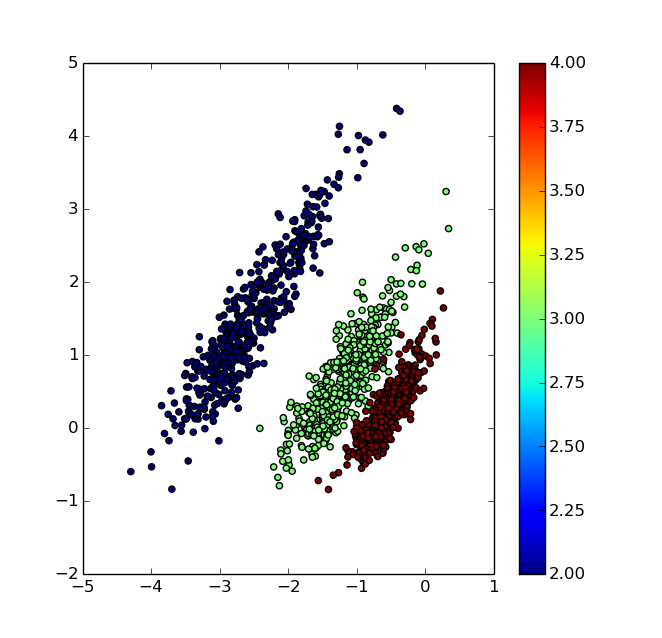
\includegraphics[width=5in]{latent_encoding.png}
\end{center}
  \caption{
The test set of causal matrices mapped into the $2$-dimensional latent space, coloured according to the dimension of the original causal sets.  
The VAE has successfully separated the three classes of causal sets, with very little overlap between them.} \label{resultsfig}
\end{figure}

\section{Future Sections} \label{future}

This is a work in progress, and using causal matrices for causal sets of different dimensions in flat spacetime was the first proof of concept of using 
VAE's to distinguish between types of causal sets.  For my next step, I intend to use causal sets with curvature in addition to the flat ones, to see if 
two latent variables are still enough to distinguish between them.  

This will be done by adding causal diamonds on de Sitter (dS) (with positive curvature) and anti-de Sitter (AdS) (with negative curvature) 
in various dimensions.  The main technical obstacle is calculating the 
shapes of the statistical distributions for the sprinklings on these spacetimes, while the autoencoder may need extra depth added in order to accommodate 
the additional complexity of the spaces.

dS and AdS are the simplest examples of curved spacetimes, since like flat spacetime, their curvature is constant at all points.  Later on, I could 
try to use spacetimes with nonconstant curvature, such as black hole or cosmological spacetimes.  A potentially exciting result would be if the VAE 
could encode all these different spacetimes using two, or at least very few, latent variables, in a way that could make it resemble a phase diagram of 
spacetimes.

Other future projects could include making the neural network more ``clever''.  Right now it will work for a causal set of fixed size only.  Ideally 
it should be able to work for causets of variable sizes.



\section{Acknowledgements}
I am grateful to Jonah Miller for suggesting this project, his helpful discussions, and recommending excellent resources.  
The variational autoencoder of Keras in \cite{kerasauto} was very valuable for this project, and was used with very little modification.

\begin{thebibliography}{99}
\bibitem{causalsets}
L.~Bombelli, J.~Lee, D.~Meyer and R.~Sorkin,
  ``Space-Time as a Causal Set,''
  Phys.\ Rev.\ Lett.\  {\bf 59}, 521 (1987).
\bibitem{vae}
D.~P.~Kingma, M.~Welling, ``Auto-Encoding Variational Bayes,'' \href{https://arxiv.org/abs/1312.6114}{https://arxiv.org/abs/1312.6114},\\
C.~Doersch, ``Tutorial on Variational Autoencoders,'' \href{https://arxiv.org/abs/1606.05908}{https://arxiv.org/abs/1606.05908}.
\bibitem{vaemnist}
F.~Cholet, ``Building Autoencoders in Keras,'' \href{https://blog.keras.io/building-autoencoders-in-keras.html}{https://blog.keras.io/building-autoencoders-in-keras.html},\\
M.~Shiffman, ``Introducing Variational Autoencoders (in Prose and Code),'' \href{http://blog.fastforwardlabs.com/2016/08/12/introducing-variational-autoencoders-in-prose-and.html}
{http://blog.fastforwardlabs.com/2016/08/12/introducing-variational-autoencoders-in-prose-and.html}
\bibitem{mnist} The MNIST Database of Handwritten Digits, \href{http://yann.lecun.com/exdb/mnist/}{http://yann.lecun.com/exdb/mnist/}.
\bibitem{kerasauto} Variational Autoencoder created by Keras team. 
 Available at \href{https://github.com/keras-team/keras/blob/master/examples/variational_autoencoder.py}{https://github.com/keras-team/keras/blob/master/examples/variational\_autoencoder.py}
\bibitem{klexplain} Comment 5 by user radek on \href{http://forums.fast.ai/t/intuition-behind-kl-divergence-regularization-in-vaes/1650/4}
{http://forums.fast.ai/t/intuition-behind-kl-divergence-regularization-in-vaes/1650/4}
\bibitem{cubetosphere} See e.g. \href{https://stats.stackexchange.com/questions/7977/how-to-generate-uniformly-distributed-points-on-the-surface-of-the-3-d-unit-sphe}{https://stats.stackexchange.com/questions/7977/how-to-generate-uniformly-distributed-points-on-the-surface-of-the-3-d-unit-sphe}
\end{thebibliography}




\end{document}